\documentclass[conference]{IEEEtran}

\usepackage{cmap}
\usepackage[utf8]{inputenc}
\usepackage[english]{babel}

\usepackage{indentfirst} 
\usepackage{amsmath,amssymb,amscd,amsthm}
\usepackage{mathtools}
%\usepackage{empheq}
%\newcommand*{\widebox}[2][0.5em]{\fbox{\hspace{#1}$\displaystyle #2$\hspace{#1}}}
%\usepackage{longtable}
\usepackage{multirow}
\usepackage{multicol}

\usepackage{graphicx}
\usepackage{caption}
\usepackage{subcaption}
\usepackage{siunitx}

\usepackage{enumitem}

\renewcommand{\sfdefault}{cmss}
\renewcommand{\rmdefault}{cmr}
\renewcommand{\ttdefault}{cmt}

\usepackage{tikz}
\usetikzlibrary{shapes,shapes.geometric,arrows,fit,calc,positioning,automata}
\usetikzlibrary{arrows}
\usetikzlibrary{shapes.multipart}
\usetikzlibrary{decorations.pathreplacing}
\usetikzlibrary{patterns}
\usetikzlibrary{arrows.meta}

\usepackage[e]{esvect}		
													
\usepackage{xcolor}
\definecolor{darkblue}{rgb}{0,0,.6}
\definecolor{Purplemountainmajesty}{RGB}{150, 120, 182}
\definecolor{prpl}{RGB}{150, 120, 182}

\interdisplaylinepenalty=2500

\pdfcompresslevel=9
\pdfobjcompresslevel=9

\usepackage{cite}
%\usepackage[breaklinks,pdftex,hyperindex,unicode]{hyperref}	
%\hypersetup{
%  pdftitle           = {IEEE 802.11ax},
%  pdfauthor          = {Didenko Andre},
%  pdfsubject         = {IEEE 802.11ax},
%  pdfstartview       = {FitH},
%  pdfborder          = {0 0 0},
%  bookmarksopen      = true,
%  bookmarksnumbered  = true,
%  bookmarksopenlevel = 2,
%  colorlinks = true,     
%  		linkcolor  = black, 
%  		urlcolor = black,
%        citecolor = black
%}

%!!!conflicting order of packages
%\usepackage{extarrows}
% fix \ordinarycolon
\edef\ordinarycolon{\mathchar\the\mathcode`:}

%\usepackage{todonotes}
%\presetkeys{todonotes}{inline, color=Purplemountainmajesty}{}

%%% my macros

%% Math fonts
\newcommand{\bbA}{\mathbb{A}}
\newcommand{\bbB}{\mathbb{B}}
\newcommand{\bbC}{\mathbb{C}} % комплексные числа
\newcommand{\bbD}{\mathbb{D}}
\newcommand{\bbE}{\mathbb{E}} 
\newcommand{\bbF}{\mathbb{F}}
\newcommand{\bbG}{\mathbb{G}}
\newcommand{\bbH}{\mathbb{H}}
\newcommand{\bbI}{\mathbb{I}}
\newcommand{\bbJ}{\mathbb{J}}
\newcommand{\bbK}{\mathbb{K}}
\newcommand{\bbL}{\mathbb{L}}
\newcommand{\bbM}{\mathbb{M}}
\newcommand{\bbN}{\mathbb{N}} %натуральные числа
\newcommand{\bbO}{\mathbb{O}}
\newcommand{\bbP}{\mathbb{P}}
\newcommand{\bbQ}{\mathbb{Q}} % рациональные числа
\newcommand{\bbR}{\mathbb{R}} % действительные числа
\newcommand{\bbS}{\mathbb{S}}
\newcommand{\bbT}{\mathbb{T}}
\newcommand{\bbU}{\mathbb{U}}
\newcommand{\bbV}{\mathbb{V}}
\newcommand{\bbW}{\mathbb{W}}
\newcommand{\bbX}{\mathbb{X}}
\newcommand{\bbY}{\mathbb{Y}}
\newcommand{\bbZ}{\mathbb{Z}} %целые числа

%Матожидание и Дисперсия. 
\newcommand{\ccM}{\mathcal{M}}
\newcommand{\ccD}{\mathcal{D}}

% Привычное написание букв каппа, эпсилон и фи и знаков "больше, или равно", "меньше, или равно", пустого множества
\renewcommand{\kappa}{\varkappa }
\renewcommand{\epsilon}{\varepsilon}
\renewcommand{\phi}{\varphi}
\renewcommand{\leq}{\leqslant}
\renewcommand{\geq}{\geqslant}
\renewcommand{\emptyset}{\varnothing}

%Возможно правильная расстановка пробелов в кванторах - НЕ ИСПОЛЬЗУЙТЕ НИ ЗА ЧТО НА СВЕТЕ, ЛУЧШЕ РУКАМИ.
\newcommand{\fa}{\quad\forall}%renewcommand возможно из-за package fontawesome, который добавляет кучу красивых символов (смайлики, рожицы, значки)
\newcommand{\ex}{\quad\exists}

%Множества с чертой:
\newcommand{\bboR}{\overline{\mathbb{R}}}
\newcommand{\bboC}{\overline{\mathbb{C}}}

%Проколотая окрестность
\newcommand{\dneio}[2]{\overset{\raisebox{0pt}[0pt][0pt]{$\scriptscriptstyle\circ$}}{O}_{#1}({#2})}
\newcommand{\dnei}[1]{\overset{\raisebox{0pt}[0pt][0pt]{$\scriptscriptstyle\circ$}}{O}({#1})}
\newcommand{\coci}[2][]{\overset{\raisebox{0pt}[0pt][0pt]{$\scriptscriptstyle\circ$}}{C^{#1}}{#2}}

% Полная производная
\newcommand{\D}[2]{\frac{d{#1}}{d{#2}}}

% Частная производная
\newcommand{\pd}[2]{\frac{\partial{#1}}{\partial{#2}}}

%%%%%%%%%%%%%%%%%%%%%%%%%%%%%%%%%%%%%%%%%%

% Действительная и мнимая части
\def\Re{\mathop{\mathrm{Re}}\nolimits}
\def\Im{\mathop{\mathrm{Im}}\nolimits}

%Ядро отображения
\def\Ker{\mathop{\mathrm{Ker}}\nolimits}

%Внутренность множества.
\DeclareMathOperator*{\interior}{int} % * предполагает использование \limits

% Носитель
\def\supp{\mathop{\mathrm{supp}}\limits}

% Дивергенция
\def\Div{\mathop{\mathrm{div}}\nolimits}

% Ротор
\def\rot{\mathop{\mathrm{rot}}\nolimits}

% Градиент
\def\grad{\mathop{\mathrm{grad}}\limits}

% Градиент
\def\argmax{\mathop{\mathrm{argmax}}\limits}

% Константа
\def\const{\mathop{\mathrm{const}}\nolimits}

% Ранг
\def\rg{\mathop{\mathrm{rg}}\nolimits}

%% Вычет
\def\res{\mathop{\rm res}\limits}

%% Расстояние
\def\dist{\mathop{\rm dist}\limits}

%% Ковариация
\def\cov{\mathop{\rm cov}\limits}

%% Интеграл в смысле главного значения
\def\v.p.{\mathop{\rm v.p.}\nolimits}

%Гиперболические функции
\def\sh{\mathop{\rm sh}\nolimits}
\def\ch{\mathop{\rm ch}\nolimits}
\def\th{\mathop{\rm th}\nolimits}

%Арктангенс
\def\arctg{\mathop{\rm arctg}\nolimits}

%Обратные гиперболические функции 
\def\arsh{\mathop{\rm arsh}\nolimits}
\def\arch{\mathop{\rm arch}\nolimits}
\def\arth{\mathop{\rm arth}\nolimits}

%%%%%%%%%%%%%%%%%%%%%%%%%%%%%%%%%%%%%%%%%%

% Крупная хи
\newcommand{\bigchi}{\text{\scalebox{1.5}{$\chi$}}}

% Римские цифры
\makeatletter
\newcommand*{\rom}[1]{\expandafter\@slowromancap\romannumeral #1@}
\makeatother

%% Text fomats
\newcommand{\tbi}[1]{\textbf{\textit{#1}}}

%% Сокращение для одной штуки

\newcommand{\Gp}{(\partial G)^{+}}

\newcommand{\Gm}{(\partial G)^{-}}










%%Это перешло сюда по наследству от теорфиза, пусть будет, мало ли. 

% Скобки (высокие)
\newcommand{\brc}[1]{\left ( {#1} \right )}

% Скобки фигурные (высокие)
\newcommand{\brcr}[1]{\left\{ {#1} \right\}}

% Скобки квадратные (высокие)
\newcommand{\brs}[1]{\left [ {#1} \right ]}

% Усреднение
\newcommand{\avg}[1]{\langle{#1}\rangle}

% Усреднение (высокое)
\newcommand{\avgh}[1]{\left\langle{#1}\right\rangle}

% Бра-вектор
\newcommand{\bra}[1]{\left\langle{#1}\right|}

% Кет-вектор
\newcommand{\ket}[1]{\left|{#1}\right\rangle}

% Скалярное произведение
\newcommand{\bk}[2]{\langle{#1}|{#2}\rangle}

% Скалярное произведение (высокое)
\newcommand{\bkh}[2]{\left\langle{#1}|{#2}\right\rangle}

% Проектор
\newcommand{\proj}[2]{\ket{#1}\bra{#2}}

% Матричный элемент
\newcommand{\bfk}[3]{\langle{#1}|{#2}|{#3}\rangle}

% Матричный элемент (высокий)
\newcommand{\bfkh}[3]{\left\langle{#1}\left|{#2}\right|{#3}\right\rangle}

% Модуль
\providecommand{\abs}[1]{\left\lvert{#1}\right\rvert}

% Норма
\providecommand{\norm}[1]{\lVert#1\rVert}

% След матрицы

\def\sp{\mathop{\mathrm{sp}}\nolimits}


\begin{document}
\IEEEoverridecommandlockouts

\title{%IEEE~802.11ax Uplink Scheduler to Minimize Delay: a Classic Problem with New Constraints
Scheduling Problem for OFDMA Uplink \\in IEEE 802.11ax Networks
\thanks{The research was supported by the Russian Science Foundation (agreement No 16-19-10687).}}

\author{
\IEEEauthorblockN{Dmitry Bankov, Andre Didenko, Evgeny Khorov, Vyacheslav Loginov, Andrey Lyakhov}
\IEEEauthorblockA{Institute for Information Transmission Problems, Russian Academy of Sciences, Moscow, Russia\\
Email: \{bankov, dida, khorov, loginov, lyakhov\}@iitp.ru}
}

\maketitle

\begin{abstract}
In the modern world to have a high-speed Internet connection is already more a necessity than a luxury. 
But in modern realities, a wireless connection does not work well in dense networks. 
So new generation of Wi-Fi devices is coming due to development of a standard IEEE 802.11ax, which should be publicly released in a couple of years. 
This new standard has the challenging goal of improving some performance indicators such as throughput per user, spectral efficiency, etc. 
It takes the best of Wi-Fi and adds technology from 4G, hence combination of both technologies will be key in designing the best performing IEEE 802.11ax solutions to scheduling problem in Wi-Fi networks. 
In this paper we investigate this problem and offer a new type of schedulers. Also we show how it is possible to adapt traditional schedulers to  IEEE 802.11ax networks.
\end{abstract}

\begin{IEEEkeywords}
Wi-Fi, IEEE 802.11ax, High Effiency WLAN, OFDMA, Scheduling
\end{IEEEkeywords}

\section{Introduction}

Wireless networks have become an indispensable thing in the modern world.
Nowadays, Wireless Local Area Network (WLAN) is believed to be the most popular technology for information transmission. 
It is not surprising. 
People can go online literally anywhere --- in a restaurant, cafe, shopping center, park, public transport, airport, at work and, of course, at home. 
The main thing is just to be within the range of the access point. 
Such popularity of this technology led to the problem of congestion of Wi-Fi networks, when one network interrupts the signal of another. 
To cope with this and many other circumstances, IEEE 802 LAN/MAN Standard committee is developing a new amelioration for Wi-Fi standard: IEEE 802.11ax (further in the paper referred to as 11ax). 

This amendment provides various ways to improve the efficiency of Wi-Fi, some of them are borrowed from 4G cellular technology. 
Nevertheless, one of the most significant enhancements of 11ax is the usa\-ge of Orthogonal Frequency-Division Multiple Access (OFDMA). 
It allows the Wi-Fi Access Point to service several stations simultaneously, to better cope with fading and, in case of uplink transmission, to improve the spectral power density.

\section{OFDMA features in 11ax}

\section{Related Works}

\section{Network Scenario and Problem Statement}

The considered Wi-Fi network scenario is shown in Fig~\ref{fig:scenario}. A group of station (STA) is associated to the Access point (AP). 

From time to time, STAs generate finite data flows to be delivered to the AP.

Stations are transmitting data in uplink using OFDMA. 

\section{Scheduling in 11ax}

можно делать. разные метрики , функции. как адаптировать известные планировщики в 11аикс в офдма. 
сртф мин задержку а другие уделывают потому что используют задержку. 

\section{Ax-adaptations of Known Schedulers}

\section{Numerical Results}

\section{Conclusion}

In the paper, we have studied scheduling problem in 11ax networks, the standard of which is currently under development.
We show that because of 11ax OFDMA peculiarities the existing schedulers cannot be directly applied to the new technology.

Specifically, in the paper we have considered the problem of uplink scheduling which aims to minimize average upload time in a scenario with high number of active users.

We showed that depending on the scenario sometimes it is worth to use classic SRTF scheduler, while in other cases the channel should be split between several STAs in order to minimize upload time.
We develop a novel scheduler, called MUTAX, which adaptively chooses the best strategy and significantly outperforms existing popular solutions.

We can get gain due to division of channel. 

\clearpage

\begin{figure*}[tb]
	\centering{
		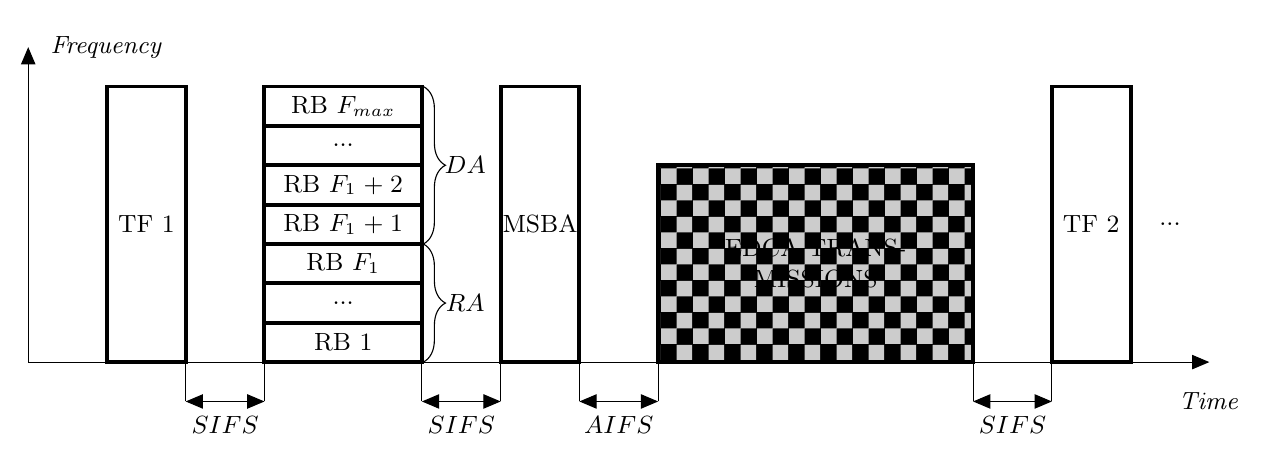
\begin{tikzpicture}
		\small
		
		\draw [arrows={-triangle 45}] (0,1) -- (15,1);
		\draw [arrows={-triangle 45}] (0,1) -- (0,5);
		\node at (15,  0.5) {\textit{Time}};
		\node at (1,  5) {\textit{Frequency}};
		
		\draw [line width=0.5mm] (1, 1) rectangle (2, 4.5);
		\node [text width=1.5cm, align=center] at (1.5,  2.75) {TF 1};
		
		\draw (2.0,  0.5) -- (2.0,  1.0);
		\draw (3.0,  0.5) -- (3.0,  1.0);
		\draw [arrows={triangle 45-triangle 45}] (2.0,0.5) -- (3.0,0.5);
		\node at (2.5, 0.2) {$SIFS$};
		
		\draw [line width=0.5mm] (3, 1.0) rectangle (5, 1.5);
		\draw [line width=0.5mm] (3, 1.5) rectangle (5, 2.0);
		\draw [line width=0.5mm] (3, 2.0) rectangle (5, 2.5);
		\draw [line width=0.5mm] (3, 2.5) rectangle (5, 3.0);
		\draw [line width=0.5mm] (3, 3.0) rectangle (5, 3.5);
		\draw [line width=0.5mm] (3, 3.5) rectangle (5, 4.0);
		\draw [line width=0.5mm] (3, 4) rectangle (5, 4.5);
		
		\node [text width=2cm, align=center] at (4, 1.25) {RB 1};
		\node [text width=2cm, align=center] at (4, 1.75) {...};
		\node [text width=2cm, align=center] at (4, 2.25) {RB $F_1$};
		\node [text width=2cm, align=center] at (4, 2.75) {RB $F_1+1$};
		\node [text width=2cm, align=center] at (4, 3.25) {RB $F_1+2$};
		\node [text width=2cm, align=center] at (4, 3.75) {...};
		\node [text width=2cm, align=center] at (4, 4.25) {RB $F_{max}$};
		
		\draw [decorate,decoration={brace,amplitude=8pt,mirror,raise=0.5pt},yshift=0pt]
		(5,1) -- (5,2.5) node [black,midway,xshift=0.55cm] {$RA$};
		\draw [decorate,decoration={brace,amplitude=8pt,mirror,raise=0.5pt},yshift=0pt]
		(5,2.5) -- (5,4.5) node [black,midway,xshift=0.55cm] {$DA$};
		
		\draw (5.0,  0.5) -- (5.0,  1.0);
		\draw (6.0,  0.5) -- (6.0,  1.0);
		\draw [arrows={triangle 45-triangle 45}] (5.0,0.5) -- (6.0,0.5);
		\node at (5.5, 0.2) {$SIFS$};
		
		\draw [line width=0.5mm] (6, 1) rectangle (7, 4.5);
		\node [text width=1.5cm, align=center] at (6.5,  2.75) {MSBA};
		
		\draw (7.0,  0.5) -- (7.0,  1.0);
		\draw (8.0,  0.5) -- (8.0,  1.0);
		\draw [arrows={triangle 45-triangle 45}] (7.0,0.5) -- (8.0,0.5);
		\node at (7.5, 0.2) {$AIFS$};
		
		\draw[draw = none,pattern=checkerboard light gray, pattern color=black, ] (8,1) rectangle (12,3.5);
		\draw [line width=0.5mm] (8, 1) rectangle (12, 3.5);
		\node [text width=3cm, align=center] at (10,  2.25) {EDCA TRANSMISSIONS};
		
		\draw (12.0,  0.5) -- (12.0,  1.0);
		\draw (13.0,  0.5) -- (13.0,  1.0);
		\draw [arrows={triangle 45-triangle 45}] (12.0,0.5) -- (13.0,0.5);
		\node at (12.5, 0.2) {$SIFS$};
		
		\draw [line width=0.5mm] (13, 1) rectangle (14, 4.5);
		\node [text width=3cm, align=center] at (13.5,  2.75) {TF 2};	
		\node [text width=1.5cm, align=center] at (14.5, 2.75) {...};
		
		\end{tikzpicture}}
	\caption{\label{fig:transmission} Frame handshake for UL OFDMA transmission.}
	\vspace{-0.5em}
\end{figure*}

\begin{figure}[b]
	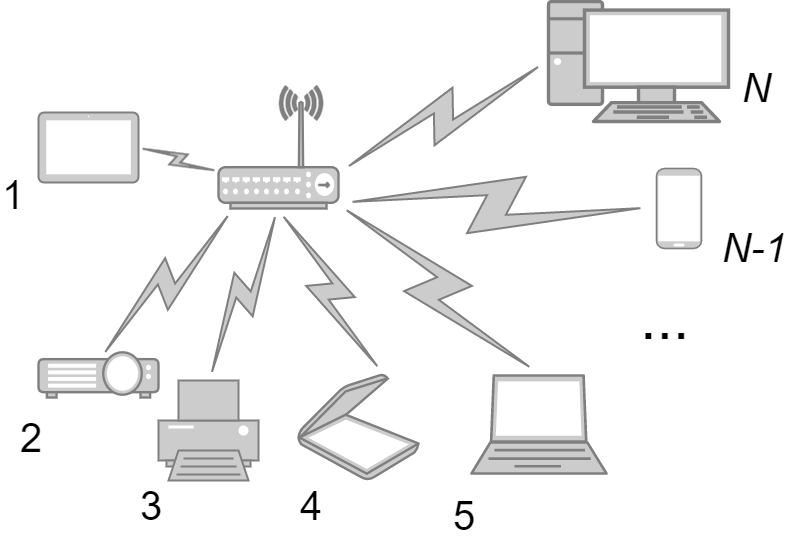
\includegraphics[width = 0.4\textwidth]{NetworkScenario}
	\caption{\label{fig:scenario} The network scenario}
\end{figure}

\begin{figure}[b]
	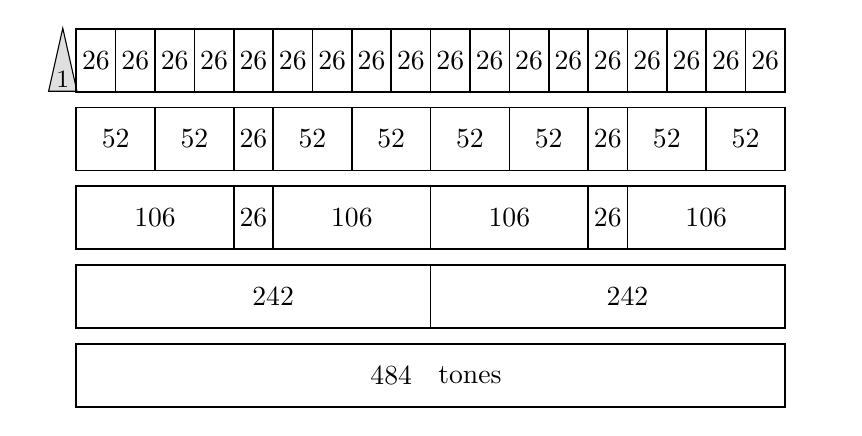
\begin{tikzpicture}[scale=1]
	
	\tikzset{primarynode/.style={isosceles triangle, draw, inner sep=0pt,
			anchor=left corner, shape border rotate=90, font=\small, fill=gray!25, isosceles triangle stretches, minimum height = 0.8cm,minimum width=0.36cm}}
	
	\node [primarynode] at (-0.36,4.0) {1};
	
	\draw [line width=0.2mm] (0.00, 0.00) rectangle (9.00, 0.80);
	\node [text width=1.5cm, align=center] at (4.0,  0.4) {484};
	\node [text width=1.5cm, align=center] at (5.0,  0.4) {tones};
	
	\draw [line width=0.2mm] (0.00, 1.0) rectangle (4.50, 1.8);
	\draw [line width=0.2mm] (4.50, 1.0) rectangle (9.00, 1.8);
	\node [text width=1.5cm, align=center] at (2.5,  1.4) {242};
	\node [text width=1.5cm, align=center] at (7.0,  1.4) {242};
	
	\draw [line width=0.2mm] (0.00, 2.0) rectangle (2.00, 2.8);
	\draw [line width=0.2mm] (2.00, 2.0) rectangle (2.50, 2.8);
	\draw [line width=0.2mm] (2.50, 2.0) rectangle (4.50, 2.8);
	\draw [line width=0.2mm] (4.50, 2.0) rectangle (6.50, 2.8);
	\draw [line width=0.2mm] (6.50, 2.0) rectangle (7.00, 2.8);
	\draw [line width=0.2mm] (7.00, 2.0) rectangle (9.00, 2.8);
	\node [text width=1.5cm, align=center] at (1.0,  2.4) {106};
	\node [text width=1.5cm, align=center] at (2.25, 2.4) {26};
	\node [text width=1.5cm, align=center] at (3.5,  2.4) {106};
	\node [text width=1.5cm, align=center] at (5.5,  2.4) {106};
	\node [text width=1.5cm, align=center] at (6.75, 2.4) {26};
	\node [text width=1.5cm, align=center] at (8.0,  2.4) {106};
	
	\draw [line width=0.2mm] (0.00, 3.0) rectangle (1.00, 3.8);
	\draw [line width=0.2mm] (1.00, 3.0) rectangle (2.00, 3.8);
	\draw [line width=0.2mm] (2.00, 3.0) rectangle (2.50, 3.8);
	\draw [line width=0.2mm] (2.50, 3.0) rectangle (3.50, 3.8);
	\draw [line width=0.2mm] (3.50, 3.0) rectangle (4.50, 3.8);
	\draw [line width=0.2mm] (4.50, 3.0) rectangle (5.50, 3.8);
	\draw [line width=0.2mm] (5.50, 3.0) rectangle (6.50, 3.8);
	\draw [line width=0.2mm] (6.50, 3.0) rectangle (7.00, 3.8);
	\draw [line width=0.2mm] (7.00, 3.0) rectangle (8.00, 3.8);
	\draw [line width=0.2mm] (8.00, 3.0) rectangle (9.00, 3.8);
	\node [text width=1.5cm, align=center] at (0.5,  3.4) {52};
	\node [text width=1.5cm, align=center] at (1.5,  3.4) {52};
	\node [text width=1.5cm, align=center] at (2.25, 3.4) {26};
	\node [text width=1.5cm, align=center] at (3.0,  3.4) {52};
	\node [text width=1.5cm, align=center] at (4.0,  3.4) {52};
	\node [text width=1.5cm, align=center] at (5.0,  3.4) {52};
	\node [text width=1.5cm, align=center] at (6.0,  3.4) {52};
	\node [text width=1.5cm, align=center] at (6.75, 3.4) {26};
	\node [text width=1.5cm, align=center] at (7.5,  3.4) {52};
	\node [text width=1.5cm, align=center] at (8.5,  3.4) {52};
	
	\draw [line width=0.2mm] (0.00, 4.0) rectangle (0.50, 4.8);
	\draw [line width=0.2mm] (0.50, 4.0) rectangle (1.00, 4.8);
	\draw [line width=0.2mm] (1.00, 4.0) rectangle (1.50, 4.8);
	\draw [line width=0.2mm] (1.50, 4.0) rectangle (2.00, 4.8);
	\draw [line width=0.2mm] (2.00, 4.0) rectangle (2.50, 4.8);
	\draw [line width=0.2mm] (2.50, 4.0) rectangle (3.00, 4.8);
	\draw [line width=0.2mm] (3.00, 4.0) rectangle (3.50, 4.8);
	\draw [line width=0.2mm] (3.50, 4.0) rectangle (4.00, 4.8);
	\draw [line width=0.2mm] (4.00, 4.0) rectangle (4.50, 4.8);
	\draw [line width=0.2mm] (4.50, 4.0) rectangle (5.00, 4.8);
	\draw [line width=0.2mm] (5.00, 4.0) rectangle (5.50, 4.8);
	\draw [line width=0.2mm] (5.50, 4.0) rectangle (6.00, 4.8);
	\draw [line width=0.2mm] (6.00, 4.0) rectangle (6.50, 4.8);
	\draw [line width=0.2mm] (6.50, 4.0) rectangle (7.00, 4.8);
	\draw [line width=0.2mm] (7.00, 4.0) rectangle (7.50, 4.8);
	\draw [line width=0.2mm] (7.50, 4.0) rectangle (8.00, 4.8);
	\draw [line width=0.2mm] (8.00, 4.0) rectangle (8.50, 4.8);
	\draw [line width=0.2mm] (8.50, 4.0) rectangle (9.00, 4.8);
	\node [text width=1.5cm, align=center] at (0.25, 4.4) {26};
	\node [text width=1.5cm, align=center] at (0.75, 4.4) {26};
	\node [text width=1.5cm, align=center] at (1.25, 4.4) {26};
	\node [text width=1.5cm, align=center] at (1.75, 4.4) {26};
	\node [text width=1.5cm, align=center] at (2.25, 4.4) {26};
	\node [text width=1.5cm, align=center] at (2.75, 4.4) {26};
	\node [text width=1.5cm, align=center] at (3.25, 4.4) {26};
	\node [text width=1.5cm, align=center] at (3.75, 4.4) {26};
	\node [text width=1.5cm, align=center] at (4.25, 4.4) {26};
	\node [text width=1.5cm, align=center] at (4.75, 4.4) {26};
	\node [text width=1.5cm, align=center] at (5.25, 4.4) {26};
	\node [text width=1.5cm, align=center] at (5.75, 4.4) {26};
	\node [text width=1.5cm, align=center] at (6.25, 4.4) {26};
	\node [text width=1.5cm, align=center] at (6.75, 4.4) {26};
	\node [text width=1.5cm, align=center] at (7.25, 4.4) {26};
	\node [text width=1.5cm, align=center] at (7.75, 4.4) {26};
	\node [text width=1.5cm, align=center] at (8.25, 4.4) {26};
	\node [text width=1.5cm, align=center] at (8.75, 4.4) {26};
	
	%\node [text width=1.5cm, align=center] at (4.5, 8.8) {DC};
	%\draw [line width=0.5mm, dashed] (4.5, 1.0) -- (4.5, 8.5);
	
	%\draw [line width=0.5mm, dashed] (0.0, 4.0) -- (0.0, 8.5);
	%\draw [line width=0.5mm, dashed] (2.0, 4.0) -- (2.0, 8.5);
	%\draw [line width=0.5mm, dashed] (2.5, 4.0) -- (2.5, 8.5);
	%\draw [line width=0.5mm, dashed] (4.5, 4.0) -- (4.5, 8.5);
	
	\end{tikzpicture}
\end{figure}

\begin{figure}[tb]
	\centering
	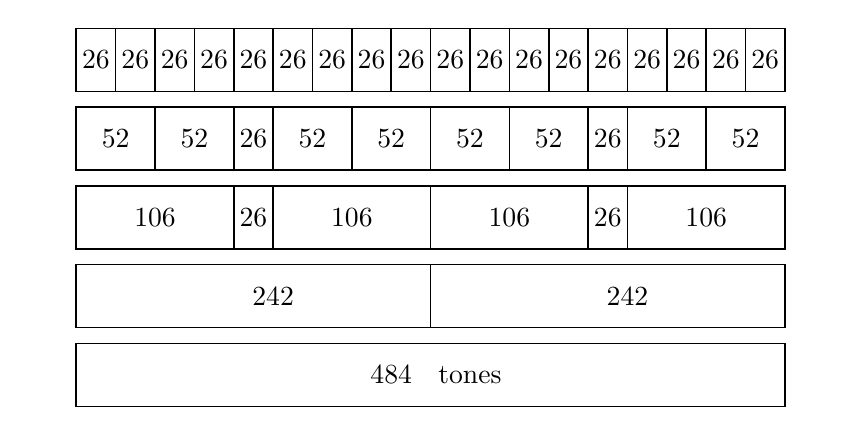
\begin{tikzpicture}[scale=1]
	
	\draw [line width=0.2mm] (0.00, 0.00) rectangle (9.00, 0.80);
	\node [text width=1.5cm, align=center] at (4.0,  0.4) {484};
	\node [text width=1.5cm, align=center] at (5.0,  0.4) {tones};
	
	\draw [line width=0.2mm] (0.00, 1.0) rectangle (4.50, 1.8);
	\draw [line width=0.2mm] (4.50, 1.0) rectangle (9.00, 1.8);
	\node [text width=1.5cm, align=center] at (2.5,  1.4) {242};
	\node [text width=1.5cm, align=center] at (7.0,  1.4) {242};
	
	\draw [line width=0.2mm] (0.00, 2.0) rectangle (2.00, 2.8);
	\draw [line width=0.2mm] (2.00, 2.0) rectangle (2.50, 2.8);
	\draw [line width=0.2mm] (2.50, 2.0) rectangle (4.50, 2.8);
	\draw [line width=0.2mm] (4.50, 2.0) rectangle (6.50, 2.8);
	\draw [line width=0.2mm] (6.50, 2.0) rectangle (7.00, 2.8);
	\draw [line width=0.2mm] (7.00, 2.0) rectangle (9.00, 2.8);
	\node [text width=1.5cm, align=center] at (1.0,  2.4) {106};
	\node [text width=1.5cm, align=center] at (2.25, 2.4) {26};
	\node [text width=1.5cm, align=center] at (3.5,  2.4) {106};
	\node [text width=1.5cm, align=center] at (5.5,  2.4) {106};
	\node [text width=1.5cm, align=center] at (6.75, 2.4) {26};
	\node [text width=1.5cm, align=center] at (8.0,  2.4) {106};
	
	\draw [line width=0.2mm] (0.00, 3.0) rectangle (1.00, 3.8);
	\draw [line width=0.2mm] (1.00, 3.0) rectangle (2.00, 3.8);
	\draw [line width=0.2mm] (2.00, 3.0) rectangle (2.50, 3.8);
	\draw [line width=0.2mm] (2.50, 3.0) rectangle (3.50, 3.8);
	\draw [line width=0.2mm] (3.50, 3.0) rectangle (4.50, 3.8);
	\draw [line width=0.2mm] (4.50, 3.0) rectangle (5.50, 3.8);
	\draw [line width=0.2mm] (5.50, 3.0) rectangle (6.50, 3.8);
	\draw [line width=0.2mm] (6.50, 3.0) rectangle (7.00, 3.8);
	\draw [line width=0.2mm] (7.00, 3.0) rectangle (8.00, 3.8);
	\draw [line width=0.2mm] (8.00, 3.0) rectangle (9.00, 3.8);
	\node [text width=1.5cm, align=center] at (0.5,  3.4) {52};
	\node [text width=1.5cm, align=center] at (1.5,  3.4) {52};
	\node [text width=1.5cm, align=center] at (2.25, 3.4) {26};
	\node [text width=1.5cm, align=center] at (3.0,  3.4) {52};
	\node [text width=1.5cm, align=center] at (4.0,  3.4) {52};
	\node [text width=1.5cm, align=center] at (5.0,  3.4) {52};
	\node [text width=1.5cm, align=center] at (6.0,  3.4) {52};
	\node [text width=1.5cm, align=center] at (6.75, 3.4) {26};
	\node [text width=1.5cm, align=center] at (7.5,  3.4) {52};
	\node [text width=1.5cm, align=center] at (8.5,  3.4) {52};
	
	\draw [line width=0.2mm] (0.00, 4.0) rectangle (0.50, 4.8);
	\draw [line width=0.2mm] (0.50, 4.0) rectangle (1.00, 4.8);
	\draw [line width=0.2mm] (1.00, 4.0) rectangle (1.50, 4.8);
	\draw [line width=0.2mm] (1.50, 4.0) rectangle (2.00, 4.8);
	\draw [line width=0.2mm] (2.00, 4.0) rectangle (2.50, 4.8);
	\draw [line width=0.2mm] (2.50, 4.0) rectangle (3.00, 4.8);
	\draw [line width=0.2mm] (3.00, 4.0) rectangle (3.50, 4.8);
	\draw [line width=0.2mm] (3.50, 4.0) rectangle (4.00, 4.8);
	\draw [line width=0.2mm] (4.00, 4.0) rectangle (4.50, 4.8);
	\draw [line width=0.2mm] (4.50, 4.0) rectangle (5.00, 4.8);
	\draw [line width=0.2mm] (5.00, 4.0) rectangle (5.50, 4.8);
	\draw [line width=0.2mm] (5.50, 4.0) rectangle (6.00, 4.8);
	\draw [line width=0.2mm] (6.00, 4.0) rectangle (6.50, 4.8);
	\draw [line width=0.2mm] (6.50, 4.0) rectangle (7.00, 4.8);
	\draw [line width=0.2mm] (7.00, 4.0) rectangle (7.50, 4.8);
	\draw [line width=0.2mm] (7.50, 4.0) rectangle (8.00, 4.8);
	\draw [line width=0.2mm] (8.00, 4.0) rectangle (8.50, 4.8);
	\draw [line width=0.2mm] (8.50, 4.0) rectangle (9.00, 4.8);
	\node [text width=1.5cm, align=center] at (0.25, 4.4) {26};
	\node [text width=1.5cm, align=center] at (0.75, 4.4) {26};
	\node [text width=1.5cm, align=center] at (1.25, 4.4) {26};
	\node [text width=1.5cm, align=center] at (1.75, 4.4) {26};
	\node [text width=1.5cm, align=center] at (2.25, 4.4) {26};
	\node [text width=1.5cm, align=center] at (2.75, 4.4) {26};
	\node [text width=1.5cm, align=center] at (3.25, 4.4) {26};
	\node [text width=1.5cm, align=center] at (3.75, 4.4) {26};
	\node [text width=1.5cm, align=center] at (4.25, 4.4) {26};
	\node [text width=1.5cm, align=center] at (4.75, 4.4) {26};
	\node [text width=1.5cm, align=center] at (5.25, 4.4) {26};
	\node [text width=1.5cm, align=center] at (5.75, 4.4) {26};
	\node [text width=1.5cm, align=center] at (6.25, 4.4) {26};
	\node [text width=1.5cm, align=center] at (6.75, 4.4) {26};
	\node [text width=1.5cm, align=center] at (7.25, 4.4) {26};
	\node [text width=1.5cm, align=center] at (7.75, 4.4) {26};
	\node [text width=1.5cm, align=center] at (8.25, 4.4) {26};
	\node [text width=1.5cm, align=center] at (8.75, 4.4) {26};
	
	%\node [text width=1.5cm, align=center] at (4.5, 8.8) {DC};
	%\draw [line width=0.5mm, dashed] (4.5, 1.0) -- (4.5, 8.5);
	
	%\draw [line width=0.5mm, dashed] (0.0, 4.0) -- (0.0, 8.5);
	%\draw [line width=0.5mm, dashed] (2.0, 4.0) -- (2.0, 8.5);
	%\draw [line width=0.5mm, dashed] (2.5, 4.0) -- (2.5, 8.5);
	%\draw [line width=0.5mm, dashed] (4.5, 4.0) -- (4.5, 8.5);
	
	\end{tikzpicture}
	\caption{\label{fig:resource_units} RU locations in \SI{40}{\MHz} channel}
	\vspace{-0.5em}
\end{figure}


\begin{table}[b]
	{\centering
		\caption{\label{table:RUdatarate} Data rate of different RU types at each MCS in Mbps}
		\resizebox{\columnwidth}{!}{
			\setlength\tabcolsep{1.5pt} % default value: 6pt
			\begin{tabular}{|c|c|c|c|c|c|c|}
				\hline
				\scriptsize\textbf{MCS}	& \scriptsize26-tone  & \scriptsize52-tone  & \scriptsize106-tone  & \scriptsize242-tone  & \scriptsize484-tone  & \scriptsize996-tone  \\
				\hline
				0	&0.8	&1.7	&3.5	&8.1 & 16.3 &34		\\
				1	&1.7	&3.3	&7.1	&16.3 & 32.5 &68.1		\\
				2	&2.5	&5	&10.6	&24.4 & 48.8 &102.1		\\
				3	&3.3	&6.7	&14.2	&32.5 & 65 &136.1		\\
				4	&5	&10	&21.3	&48.8 & 97.5 &204.2		\\
				5	&6.7	&13.3	&28.3	&65 & 130 &272.2		\\
				6	&7.5	&15	&31.9	&73.1 & 146.3 &306.3		\\
				7	&8.3	&16.7	&35.4	&81.3 & 162.5 &340.3		\\
				8	&10	&20	&42.5	&97.5 & 195 &408.3		\\
				9	&11.1	&22.2	&47.2	&108.3 & 216.7 &453.7		\\
				10	& --	&--	&--	&121.9 & 243.8 &510.4		\\
				11	& --	&--	&--	&135.4 & 270.8 &576.1		\\
				\hline
			\end{tabular}
		}
	}
\end{table}

\clearpage

\section{Main features of OFDMA in 11ax}
Data transmission in Wi-Fi with OFDMA has a number of peculiarities which make it different from data transmission in 4G, although it also uses OFDMA.

\subsection{Channelization in 802.11ax}
The available channel can be split into sets of OFDMA subcarriers called resource units (RUs).
The 11ax defines RUs that consist of 26, 52, 106, 242, 484, 996 and $2\times996$ OFDM tones.
The set of available RUs depends on the channel width, e.g., in a \SI{40}{\MHz} channel the STAs can use RUs with up to 484 tones.
A wide RUs can be split into narrower RUs: 52-tone, 106-tone RU and 484-tone RUs can be split in two approximately twice-narrower RUs from available set, while 242-tone and 996-tone RUs are split into three RBs (see Fig.~\ref{fig:resource_units}). 

The scheduler can allocate only one RU to a station, but it can vary the RU size for each station according to the aforementioned limitations.
In other words we have 37 26-tone resource units and certain groups of 2, 4, 9, 18 or all 37 of them can be united in order to obtain larger RUs.
According to the standard, such a limitation appears because of the need to have service tones next to each allocated RU of any size. 
Note, that position of these divided RBs is declared in standard and can't be arbitrary.
For example, as shown at Fig.~\ref{fig:resource_units} two first RUs are united in one 52-tone RU, 

The size of an RU determines the set of modulation-coding schemes (MCSs) that can be used for transmission in the RU.
For example, the standard prohibits the usage of high-speed MCSs in small RUs.
At the same time, for each RU width, the standard defines the minimal receiver sensitivity to signal transmitted with a specific MCS, and the faster the MCS, the higher is the sensitivity threshold.
As the result, a STA cannot use high-speed MCSs if it has poor channel conditions.

A wider RU does not necessarily mean that the STA transmits at greater speed.
A STA uses the same transmission power both for wide and narrow RUs, which results in greater signal-to-noise ratio ($SNR$) values for narrow RUs.
As the result, in a narrow RU it can use higher MCSs which can yield greater transmission rate.

\section{OFDMA SLAVA}

For an OFDMA transmission, the AP can split the whole
bandwidth into several resource units (RUs). An RU can
contain 26, 52, 106, 242, 484 or 996 tones (including service
ones). The whole 20 MHz band, 40 MHz band, 80 MHz band
and 160 (80+80) MHz band correspond to a 242-tone RU, 484-
tone RU, 996-tone RU and two 996-tone RUs, respectively.
Every RU can be split into two approximately twice-narrower
RUs. In turn, each of them can be split again, separately from
another one, with the following exception. A 996-tone RU can
be split into two 484-tone RUs and one 26-tone RU, while a
242 RU can be split into two 106-tone RUs and one 26-tone
RU. Thus, RUs can be very flexibly allocated, and the AP
should try to serve simultaneously as many STAs as it has.

Though OFDMA can be used for both UL and DL, UL
transmissions and DL transmissions cannot overlap.

For DL OFDMA transmission, the AP just sends a packet
with a common preamble and RU-dependent payload. The
information about addresses and allocation of the RUs is
indicated at the beginning of the frame.

UL OFDMA transmission is more challenging, since
OFDMA transmissions of each STAs shall start and end
simultaneously. That is why it starts with a trigger frame in
which the AP allocates RUs to each STA and informs the
STAs about the transmission parameters, e.g. MCS, transmission
duration. Being polled with the trigger frame, each
STA immediately replies with a data frame. The amendment
describes several ways how to meet the requirement on the
transmission duration. For example, advanced aggregation and
fragmentation methods, as well as padding, can be used. After
the UL transmission, the AP replies with a modified ACK
frame, in which the AP acknowledges successfully received
packets or fragments. To notify the AP that the STA has
some data for transmission, it can send a buffer status report
with the legacy channel access method, or as a part of the
described UL OFDMA transmission, or using ALOHA-like
Random OFDMA channel access, which is efficient only for
short transmissions and is not considered in the paper.

\section{OFDMA in IEEE 802.11ax Networks}
\label{sec:ofdma}
\subsection{Main Features}
\label{mainfeatures}
%main peculiarities of OFDMA in Wi-Fi

%How it differs from LTE ones

%Why it can be fruitful

%One of the most loved Wi-Fi features is backward compatibility. Several Wi-Fi generations have passed (IEEE 802.11a/b/g/n/ac), but still different generation Wi-Fi devices are capable to efficiently and fairly share common radio resources.

In contrast to LTE with a rigid traffic-independent time-frequency numerology, in 11ax networks, OFDMA works at the per-frame bases upon native to Wi-Fi Enhanced Distributed Channel Access (EDCA), a sort of decentralized CSMA/CA joint with automatic repeat request. OFDMA frames start with a common preamble, which can be decoded by legacy devices. Having received the preamble, a STA learns the duration of the frame and considers the medium as busy till the end of the frame.
The rest of the frame --- understandable only by 11ax STAs --- can be formed according to OFDMA concept, i.e. various tones of the frame can be assigned to different STAs. 

In 11ax networks, a group of tones assigned to a STA is called Resource Unit (RU).
The IEEE 802.11ax defines RUs that consist of 26, 52, 106, 242, 484, 996 and $2\times996$ OFDM tones.
The set of available RUs depends on the channel width, e.g., in a \SI{40}{\MHz} channel, the STAs can use RUs of up to 484 tones.
A wide RUs can be split into approximately twice narrower RUs \textit{independently from others}. The two exceptions are as follows.
1) A 996-tone RU can be split into two 484-tone RU and one 26-tone RU.
2) A 242-tone RU can be split into two 106-tone RU and one 26 tone RU, see Fig.~\ref{fig:resource_units}.

In LTE networks, a scheduler can allocate an arbitrary subset of downlink (DL) RUs for a user or an arbitrary \emph{interval} of UL RUs for a user.
11ax imposes much stricter constrains on RU selection, since both in DL and UL, a STA cannot be assigned to more than one RU.

Another set of constraints limits the maximal MCS that can be used in narrow RUs and the usage of MU MIMO.
Specifically, MU MIMO is only available in 106-tone and greater RUs, while the novel 1024QAM can be used only in 242-tone and greater RUs.
Such constraints complicate scheduling problem in 11ax networks.

An OFDMA frame may contain RUs with different number of tones, however all RUs inside the frame must have the same duration.
For that, the STAs may use novel flexible fragmentation or padding. 

All transmissions inside one OFDMA frame must be synchronized, i.e. start and finish at the same time instants.
This can be easily done in DL, where an OFDMA frame is generated by the Access Point (AP).
However, to provide synchronization for uplink, the AP can use novel Trigger Frame (TF).
SIFS after TF reception, the STAs transmit their parts of UL OFDMA frame.
If needed, the AP acknowledges reception of each part by sending a set of ACKs inside an OFDMA frame or by sending Multi-STA Block Acknowledgment (MSBA).

It is the AP which, for both DL and UL transmissions, determines modulation and coding scheme (MCS), duration, RU assignment and other OFDMA parameters. Such information can be transmitted in frame headers (for DL) and in the Trigger frame (for UL). An example of UL OFDMA transmission is shown in Fig.~\ref{fig:transmission}. 

As mentioned above, 11ax moves decision making logic from the STAs to the AP that determines which STA transmits, when, in which RU, how much data it transmits, etc.
To make a correct decision, the AP needs to be aware of STAs' buffered traffic and channel conditions.
This information can be periodically requested by the AP.
Moreover, to notify the AP about arrived packets, a STA can proactively send so-called Buffer Status Report (BSR).
For that, it can aggregate BSR with a data frame sent in the dedicated RU.
Another option is legacy EDCA.
Thanks to the recent change in the 11ax draft standard, the AP can separately tune EDCA parameters of scheduled STAs in such a way, that they do not contend for the channel with unscheduled STAs.
It means that if a STA does not obtain UL RUs, it likely delivers a BSR at the first transmission attempt because of the extremely low contention.
The third approach to send a BSR is using OFDMA Random Access.
For that, the AP can allocate one or several RUs for random access and the contending STAs will randomly choose one of such RUs. 
Anyway, thanks to these methods, the AP can quickly obtain information about new frames buffered  at the associated STAs and waiting for UL RUs.

OFDMA brings many benefits to 11ax networks.
First it makes transmission more reliable to frequency selective interference and fading.
This is especially important for wide \SI{160}{MHz} channels introduced in 11ac.
Second, with OFDMA we can glue short packets destined for or originated from various STAs, which significantly reduces overhead caused by PHY headers and channel access time and interframe spaces.
Third, for UL transmissions by edge STAs it makes sense to use narrow channels instead of wide ones.
Indeed, since the STAs are spatially separated they can simultaneously transmit at the maximal allowed power without breaking legal limitations on the emitted energy.
Thus, by reducing RU width, we increase power spectral density received from the STAs and can use higher MCS.
In other words, by allowing numerous spatially separated STAs to transmit in parallel, we increase the cumulative received power in comparison to the case when only one STA transmits.
For edge STAs, increasing power spectral density leads to a higher MCS, so  the average amount of data received from an OFDMA frame is higher than that from a legacy.
Thus in contrast to LTE, in 802.11ax networks the rates in UL RUs are non-additive, i.e. if a STA transmits in twice wider RU, it is not guaranteed that it transmits twice more data.
This effect will be carefully investigated in the paper.

While in DL OFDMA just allows AP to transmit data to multiple users simultaneously, OFDMA in the uplink provides more benefits. In particular, independently on the size of RU in which STA is transmitting, STA spends the same amount of power $P_0$. Because of that, with OFDMA the signal power density is increased, so MCS with higher data rate can be used for transmission in narrower RU. As a result, in contrast to LTE, in 802.11ax uplink transmission data rate in different RUs is non-additive, i.e. if a STA transmits in twice wider RU, it is not guaranteed that it achieves twice higher data rate. Moreover, in some cases the achieved data rate can be even smaller.

Data rates of MCSs used in the 802.11ax are indicated in Table~\ref{table:RUdatarate}.

\clearpage
\section{CONTINIYTUE}
\subsection{Data Transmission Sequence}
To organize data transmission process with OFDMA, the AP transmits Trigger Frames, in which it includes the scheduling information (see Fig. \ref{fig:transmission}).
Specifically, for each allocated RU it adds a User Info element that indicates the RU, the MCS that should be used in that RU and the AID of the designated STA.
If the AID is $0$, then the RU is allocated for random access, which can be used by STAs to request channel resources from the AP.

Having received a Trigger Frame, STAs transmit their data frames in designated RUs or in RUs allocated for random access.
The inter-frame space between the STAs' frames and the Trigger Frame is $SIFS$.
The STAs pad their frames, so that they end at the same time.
To acknowledge the STA transmissions, the AP can either send multiple BlockAcks in each RU to the respective STAs, or send a single Multi-STA BlockAck which acknowledges the frames from all STAs.
In any case, the inter-frame space used is $SIFS$

\subsection{Random Access with Wi-Fi OFDMA}
The AP includes in beacons an OFDMA-based Random Access Parameter Set element, which contains the OFDMA contention window ($OCW$) parameters, specifically, its minimal ($OCWmin$) and maximal ($OCWmax$) values.

To transmit a frame in random access, a STA maintains an OFDMA backoff (OBO) counter and an OFDMA contention window, initially equal to $OCWmin$.
For a frame transmission, the STA draws its OBO counter equiprobably in the range from $0$ to $OCW$.
Every time a STA receives a Trigger Frame, it decrements the OBO counter by the number of RUs assigned for random access.
If the OBO counter becomes less then or equal to zero, the STA randomly selects one of the RUs assigned for random access and transmits its frame in this RU.
If the frame is successfully transmitted (i.e., the STA has received an acknowledgement for its frame), the STA sets its $OCW$ to $OCWmin$.
Otherwise, the STA updates its $OCW$ to $2 \times OCW + 1$, if the new $OCW$ does not exceed $OCWmax$.

\section{Related Papers}
Reviews: \cite{khorov2015ieee, bellalta2016ieee}.
Performance improvement for random access: \cite{khorov2016several}.
Dense deployment interference improvement: \cite{khorov2016joint}.
Something about OFDMA: \cite{qu2015ofdma}.

\section{Network Scenario and Problem Statement}
We consider a scenario with an AP and a group of STAs connected to it.
From time to time STAs generate data streams that have to be transmitted to the AP.
The data stream length in bytes and the interval between two stream generation times are random and are described by a given distribution.
In the considered scenario devices use only OFDMA for data transmission, i.e., traditional Wi-Fi random access (EDCA) is not used.

When a STA generates a stream, it requests channel resources from the AP.
For this purpose it uses the OFDMA random access to send a buffer status report (BSR) to the AP.
Having received a BSR, the AP learns that it has to allocate an RU for the STA, and also it learns the amount of resources that the STA intends to transmit.

We consider a typical scenario for uplink data transmission in Wi-Fi network, when the STAs send small streams, such as HTML requests or any other data related to Web browsing.
In such scenario, it is critical to minimize the data delivery time for the STAs.
The data delivery time for the STAs depends on two summands: the time spent in random access and the time spent actually transmitting data.
Both of these summands are, in fact, determined by the scheduling algorithm used at the AP.

The IEEE 802.11ax standard does not specify a scheduler.
It does not state the number of RUs that should be allocated for random access, neither does it define an algorithm to select the RU sizes for different STAs.

So we state the following problem in the paper: \emph{to design a scheduler for Wi-Fi OFDMA uplink data transmission that minimizes data delivery time}.

\section{Scheduler}
Dynamic programming algorithm to solve the problem: \cite{bourgeois1971extension}.
\section{Extra information}

We need to make a few preliminary remarks. If sender have a small amount of data. We consider uplink traffic. That's why we can 

When stations should request a frequency band

\clearpage

\clearpage

\begin{abstract}
	In order to meet the continuously increasing demands for high throughput in wireless networks, IEEE 802 LAN/MAN Standard Committee is developing IEEE 802.11ax: a new amendment for the Wi-Fi standard.
	This amendment provides various ways to improve the efficiency of Wi-Fi. The most revolutionary one is OFDMA.
	Apart from obvious advantages, such as decreasing overhead for short packet transmission at high rates and improving robustness to frequency selective interference, being used for uplink transmission, OFDMA can increase power spectral density and, consequently, user data rates. However, the gain of OFDMA mainly depends on the resource scheduling between users.
	%It allows the Wi-Fi Access Point to service several stations simultaneously, to better cope with fading and, in case of uplink transmission, to improve the spectral power density.
	The peculiarities of OFDMA implementation in Wi-Fi completely change properties of classic schedulers used in other OFDMA systems, e.g. LTE. 
	In the paper, we consider the usage of OFDMA in Wi-Fi for uplink transmission.
	We study peculiarities of OFDMA in Wi-Fi, adapt classic schedulers to Wi-Fi, explaining why they do not perform well.
	Finally we develop a novel scheduler, MUTAx, and evaluate its performance with simulation. 
\end{abstract}

\begin{IEEEkeywords}
	Wi-Fi, IEEE 802.11ax, High Effiency WLAN, OFDMA, Scheduling
\end{IEEEkeywords}

\section{Introduction}
%According to Cisco report, 50\% of traffic will be transmitted over WLANs in 2021 \cite{ciscoreport}. 
Nowadays, Wi-Fi has become the main technology for wireless local area networks. High number of Wi-Fi devices, as well as the number of deployed networks, leads to huge interference. To improve efficiency of Wi-Fi networks in existing and emerging indoor and outdoor scenarios, Wi-Fi community is currently developing a new standard, namely IEEE 802.11ax. 
In contrast to 11ac, PHY layer data rate of which tenfold excels the one of the preceding technology (namely 11n), the expected quadruple growth of user throughput in 11ax networks will be caused mostly by advanced channel access techniques, rather than by PHY data rates increased by just 37\%.

The main feature of 11ax is Orthogonal Frequency Division Multiple Access (OFDMA), which extends the legacy Wi-Fi Carrier Sense Multiple Access with Collision Avoidance (CSMA/CA) by introducing a possibility to divide channel resources in frequency domain. Since 11a, Wi-Fi has been using Orthogonal Frequency Division Multiplexing (OFDM). However, with OFDM, at any time instant all tones (also referred to as subcarriers) are used to transmit data for one user, while OFDMA allows assigning various tones to different users. The efficiency of OFDMA significantly depends on how the tones are scheduled between users. However the 11ax standard will provide only a flexible framework, without any predefined scheduling algorithms. 

Fortunately, scheduling problem has been carefully investigated in cellular networks, like LTE, where OFDMA has appeared much earlier. So at first sight, it is worth to use one of the existing cellular schedulers and adapt it to Wi-Fi peculiarities. This work itself is not easy, since OFDMA fundamentals in Wi-Fi differ from that in LTE. Moreover, the features of 11ax break assumptions used to derive schedulers for LTE. Thus, nobody can guarantee that being applied to 11ax networks the LTE scheduler remain the best one. 

In this paper, we compare OFDMA schemes in IEEE 802.11ax and LTE, and analyze problems that arise while developing the schedulers for 11ax networks. We also make the first step in this direction and consider a problem of minimizing the average delivery time for uplink transmission. Then we show why well-known schedulers designed for a similar problem are not optimal for 11ax networks and develop a new scheduler that outperforms them. 

The rest of the paper is organized as follows.
Section~\ref{sec:ofdma} briefly describes the main features of OFDMA in 802.11ax, reviews literature and states the problem.
In Section \ref{mutex} we design a brand new scheduler for 11ax networks.
We prove its high efficiency in Section \ref{numerical}.
Section~\ref{conclusion} concludes the paper. 



\section{OFDMA in IEEE 802.11ax Networks}
\label{sec:ofdma}
\subsection{Main Features}
\label{mainfeatures}
%main peculiarities of OFDMA in Wi-Fi

%How it differs from LTE ones

%Why it can be fruitful

%One of the most loved Wi-Fi features is backward compatibility. Several Wi-Fi generations have passed (IEEE 802.11a/b/g/n/ac), but still different generation Wi-Fi devices are capable to efficiently and fairly share common radio resources.

In contrast to LTE with a rigid traffic-independent time-frequency numerology, in 11ax networks, OFDMA works at the per-frame bases upon native to Wi-Fi Enhanced Distributed Channel Access (EDCA), a sort of decentralized CSMA/CA joint with automatic repeat request. OFDMA frames start with a common preamble, which can be decoded by legacy devices. Having received the preamble, a STA learns the duration of the frame and considers the medium as busy till the end of the frame.
The rest of the frame --- understandable only by 11ax STAs --- can be formed according to OFDMA concept, i.e. various tones of the frame can be assigned to different STAs. 

In 11ax networks, a group of tones assigned to a STA is called Resource Unit (RU).
The IEEE 802.11ax defines RUs that consist of 26, 52, 106, 242, 484, 996 and $2\times996$ OFDM tones.
The set of available RUs depends on the channel width, e.g., in a \SI{40}{\MHz} channel, the STAs can use RUs of up to 484 tones.
A wide RUs can be split into approximately twice narrower RUs \textit{independently from others}. The two exceptions are as follows.
1) A 996-tone RU can be split into two 484-tone RU and one 26-tone RU.
2) A 242-tone RU can be split into two 106-tone RU and one 26 tone RU, see Fig.~\ref{fig:resource_units}.

In LTE networks, a scheduler can allocate an arbitrary subset of downlink (DL) RUs for a user or an arbitrary \emph{interval} of UL RUs for a user.
11ax imposes much stricter constrains on RU selection, since both in DL and UL, a STA cannot be assigned to more than one RU.

Another set of constraints limits the maximal MCS that can be used in narrow RUs and the usage of MU MIMO.
Specifically, MU MIMO is only available in 106-tone and greater RUs, while the novel 1024QAM can be used only in 242-tone and greater RUs.
Such constraints complicate scheduling problem in 11ax networks.

An OFDMA frame may contain RUs with different number of tones, however all RUs inside the frame must have the same duration.
For that, the STAs may use novel flexible fragmentation or padding. 

All transmissions inside one OFDMA frame must be synchronized, i.e. start and finish at the same time instants.
This can be easily done in DL, where an OFDMA frame is generated by the Access Point (AP).
However, to provide synchronization for uplink, the AP can use novel Trigger Frame (TF).
SIFS after TF reception, the STAs transmit their parts of UL OFDMA frame.
If needed, the AP acknowledges reception of each part by sending a set of ACKs inside an OFDMA frame or by sending Multi-STA Block Acknowledgment (MSBA).

It is the AP which, for both DL and UL transmissions, determines modulation and coding scheme (MCS), duration, RU assignment and other OFDMA parameters. Such information can be transmitted in frame headers (for DL) and in the Trigger frame (for UL). An example of UL OFDMA transmission is shown in Fig.~\ref{fig:transmission}. 

As mentioned above, 11ax moves decision making logic from the STAs to the AP that determines which STA transmits, when, in which RU, how much data it transmits, etc.
To make a correct decision, the AP needs to be aware of STAs' buffered traffic and channel conditions.
This information can be periodically requested by the AP.
Moreover, to notify the AP about arrived packets, a STA can proactively send so-called Buffer Status Report (BSR).
For that, it can aggregate BSR with a data frame sent in the dedicated RU.
Another option is legacy EDCA.
Thanks to the recent change in the 11ax draft standard, the AP can separately tune EDCA parameters of scheduled STAs in such a way, that they do not contend for the channel with unscheduled STAs.
It means that if a STA does not obtain UL RUs, it likely delivers a BSR at the first transmission attempt because of the extremely low contention.
The third approach to send a BSR is using OFDMA Random Access.
For that, the AP can allocate one or several RUs for random access and the contending STAs will randomly choose one of such RUs. 
Anyway, thanks to these methods, the AP can quickly obtain information about new frames buffered  at the associated STAs and waiting for UL RUs.

OFDMA brings many benefits to 11ax networks.
First it makes transmission more reliable to frequency selective interference and fading.
This is especially important for wide \SI{160}{MHz} channels introduced in 11ac.
Second, with OFDMA we can glue short packets destined for or originated from various STAs, which significantly reduces overhead caused by PHY headers and channel access time and interframe spaces.
Third, for UL transmissions by edge STAs it makes sense to use narrow channels instead of wide ones.
Indeed, since the STAs are spatially separated they can simultaneously transmit at the maximal allowed power without breaking legal limitations on the emitted energy.
Thus, by reducing RU width, we increase power spectral density received from the STAs and can use higher MCS.
In other words, by allowing numerous spatially separated STAs to transmit in parallel, we increase the cumulative received power in comparison to the case when only one STA transmits.
For edge STAs, increasing power spectral density leads to a higher MCS, so  the average amount of data received from an OFDMA frame is higher than that from a legacy.
Thus in contrast to LTE, in 802.11ax networks the rates in UL RUs are non-additive, i.e. if a STA transmits in twice wider RU, it is not guaranteed that it transmits twice more data.
This effect will be carefully investigated in the paper.

While in DL OFDMA just allows AP to transmit data to multiple users simultaneously, OFDMA in the uplink provides more benefits. In particular, independently on the size of RU in which STA is transmitting, STA spends the same amount of power $P_0$. Because of that, with OFDMA the signal power density is increased, so MCS with higher data rate can be used for transmission in narrower RU. As a result, in contrast to LTE, in 802.11ax uplink transmission data rate in different RUs is non-additive, i.e. if a STA transmits in twice wider RU, it is not guaranteed that it achieves twice higher data rate. Moreover, in some cases the achieved data rate can be even smaller.

Data rates of MCSs used in the 802.11ax are indicated in Table~\ref{table:RUdatarate}.

\subsection{Data Transmission Sequence}
To organize data transmission process with OFDMA, the AP transmits Trigger Frames, in which it includes the scheduling information (see Fig. \ref{fig:transmission}).
Specifically, for each allocated RU it adds a User Info element that indicates the RU, the MCS that should be used in that RU and the AID of the designated STA.
If the AID is $0$, then the RU is allocated for random access, which can be used by STAs to request channel resources from the AP.

Having received a Trigger Frame, STAs transmit their data frames in designated RUs or in RUs allocated for random access.
The inter-frame space between the STAs' frames and the Trigger Frame is $SIFS$.
The STAs pad their frames, so that they end at the same time.
To acknowledge the STA transmissions, the AP can either send multiple BlockAcks in each RU to the respective STAs, or send a single Multi-STA BlockAck which acknowledges the frames from all STAs.
In any case, the inter-frame space used is $SIFS$




\subsection{Random Access with Wi-Fi OFDMA}
The AP includes in beacons an OFDMA-based Random Access Parameter Set element, which contains the OFDMA contention window ($OCW$) parameters, specifically, its minimal ($OCWmin$) and maximal ($OCWmax$) values.

To transmit a frame in random access, a STA maintains an OFDMA backoff (OBO) counter and an OFDMA contention window, initially equal to $OCWmin$.
For a frame transmission, the STA draws its OBO counter equiprobably in the range from $0$ to $OCW$.
Every time a STA receives a Trigger Frame, it decrements the OBO counter by the number of RUs assigned for random access.
If the OBO counter becomes less then or equal to zero, the STA randomly selects one of the RUs assigned for random access and transmits its frame in this RU.
If the frame is successfully transmitted (i.e., the STA has received an acknowledgement for its frame), the STA sets its $OCW$ to $OCWmin$.
Otherwise, the STA updates its $OCW$ to $2 \times OCW + 1$, if the new $OCW$ does not exceed $OCWmax$.


\subsection{Related Works}

Despite the fact that 802.11ax amendment is expected to be finished by 2019, it has been already studied in the literature\cite{ bellalta2016ieee, khorov2016several, karaca2016resource, ofdma-par1, ofdma-par2}.

In \cite{khorov2016several}, authors study the performance of the network consisting of the legacy and 802.11ax STAs.
Authors propose an approach for optimal channel access parameter values selection, which guarantees fairness between legacy and 802.11ax and significantly increases the number of the OFDMA transmissions for 802.11ax STAs.
However, the model developed in \cite{khorov2016several} allows only estimating the number of the OFDMA transmissions in the network, but not the achievable data rate.

Many studies on 802.11ax performance were presented at the meetings of the 802.11ax Task Group (TGax), e.g. \cite{ofdma-par1, ofdma-par2}.
However, although many network topologies have been already studied, the only considered scheduler in TGax has been the random scheduler with a static RU configuration.

The problem of scheduling in 11ax uplink has been considered in \cite{karaca2016resource}, which focuses on selection of the RU duration.
The authors initially assume that the AP does not know the amount of data the STAs have and thus does not know the correct duration of RUs that should be allocated.
They propose a scheme that can be used by the AP to obtain this information and derive the best way to select the duration of STAs' transmission in terms of throughput and energy consumption.
However, they do not consider any specific way to divide the channel into RUs and to assign the RUs to the STAs.
Neither do they consider random access and the possibility of STAs to deliver RSRs by aggregating them to the transmitted data.

%Dense deployment interference improvement: \cite{khorov2016joint}.

Random access for UL OFDMA in 802.11ax has been studied in \cite{lanante2017performance}.
The authors consider a scenario, when STAs transmit saturated data flows and use only random access for transmission.
They describe a mathematical model of transmission with OFDMA random access and use it for analysis and optimization of the network performance in terms of throughput and percentage of successful RUs.
The methodology introduced in the paper might be used to tune the random access for OFDMA UL, however, usage of deterministic access is more feasible in terms of channel efficiency for the studied scenario.

The problem of resource allocation in cellular networks is widely studied in literature.
In many papers, it is formulated as the following optimization problem.
Consider a network with a base station (BS) and $N$ associated users.
Each time unit, the BS runs scheduler which allocates $M$ RUs to some STAs in order to maximize some network-wide utility function.
The most widely used utility functions and corresponding schedulers are listed below. 

To maximize cumulative throughput $S = \sum\limits_{i=1}^N S_i(t)$ at time instant $t$, the BS uses the Max Rate (MR) scheduler, which considers RUs one by one and assigns each RU to a user with the highest nominal data rate $r_{i}^{j}$ in this RU.
However, as shown in many papers (e.g. \cite{capozzi2013downlink}), under high load the MR scheduler blocks users with low instant rates.

To avoid this problem, the Proportional Fair (PF) scheduler has been proposed.
It maximizes $\sum_{i=1}^{N} \log{S_i(t)}$.
For that, RU $j$ shall be allocated to user $\hat{i}_{PF}= \arg \max_i \frac{r_i^{(j)}(t)}{S_{i}(t-1)}.$
Authors of~\cite{kwan2009proportional} show that in long term the PF scheduler gives the same amount of channel time for all users, therefore resulting in fair resource allocation.

Both MR and PF have been designed for saturated (infinite) flows.
From the practical point of view, it is worth to consider unsaturated scenario with finite flows of given length.
Such flows can represent HTTP requests or files transmitted in a wireless network.
For such traffic, it is worth to consider upload time which affects user perceived quality of experience (QoE).
If the channel properties do not change with time, the rate in different RUs is the same and additive, the Shortest Remaining Time First (SRTF) scheduler is proven to provide minimal average upload time.
Simplistically, SRTF allocates all RUs to a user for which $\frac{D_i(t)}{r_i}$ is the minimal one, where $D_i(t)$ is the remaining amount of data of user $i$ and $r_i$ is its rate in the whole channel.
As explained in Section \ref{mainfeatures}, the assumptions made to derive such a scheduler are not met for UL OFDMA transmission in 11ax networks, which brings us to the following problem statement.


\section{Design of the Scheduler}
\label{mutex}
In this section, we design a novel scheduler called MUTAX, Minimizing Upload Time in 11AX networks. While deriving formulae we neglect the effects related to packetization (including aggregation and fragmentation) overhead. Apart from that, for shortness we consider only $n$ STAs with flows and assume that each STA has only one flow. Both STA and flow are denoted as $i, i=1,...,n$.

Let slot be a time interval between two consequent TFs.
It should be noted that slots may have different duration. The maximal one is related to the standard limit of \SI{5484}{\us} for the physical protocol data unit (PPDU) duration. A slot can be shorter, if at least one STA which transmits in this slot has no more data.

The MUTAX algorithm has two steps. At the first step, we order existing flows and calculate the sum upload time of the flows, as if we used exhaustive service.
At the second stage, we try to improve the sum upload time by serving some flows in parallel.
Let us consider the steps in detail.

At the first step, we serve each flows exhaustively.
Except for waiting, the time needed to upload flow $i$ equals $t_i = \frac{D_i}{r_{i}}$. %, where $r_{i}$ is the rate of STA $n$ transmitting in the whole frequency channel.
The first STA finishes delivering its flow by time $t_1$.
The second STA starts right after the first one and delivers its flow by time $t_2 + t_1$, etc.
As the result, the total upload time for existing flows is
\[ T_{step1} = \sum_{i = 1}^{n} \left(n - i\right) t_i. \]
Obviously, to minimize the sum upload time we have to sort the STAs in the ascending order by $t_i$.

At the second step, we divide the channel into several RUs.   
Let $m$ be the number of RUs and $j, 1\le j \le m$ be the index of RU in the considered RU configuration.  
$x_i^j$ is an indicator which equals $1$ if STA $i$ is assigned to RU $j$, and $0$, otherwise.
For shortness, $X$ is the two dimensional matrix of $\left\{x_i^j\right\}$ representing RU assignment to the STAs. 

With defined notation, the total upload time $T\left(X\right) $ of existing flows differs from $T_{step1}$ in the following way. First, the upload time of each of $n$ flows increases by  the current slot duration $\tau$. Second, if $x_i^j=1$, the remaining amount of data of flow $i$ decreases by the amount of data the STA transmits in RU $j$ of the current slot: $\Delta D_i^j = \min\left\{D_i, \tau \times r_{i}^{j}\right\}$. Thus  
\[ T\left(X\right) = n \tau + \sum_{i = 1}^{n} \left(n - i\right) \frac{D_i -  \sum_{k = 1}^{m} x_i^j \Delta D_i^j}{r_{i}} \]


%Leaving out of consideration $n \tau_t$, we can say that to minimize $T\left(X\right)$ we need to sort STAs in the ascending order by $\frac{D_i -  \sum_{k = 1}^{m} x_i^j \Delta D_i^j}{r_{i}}$.

Since both $\tau$ and  $\Delta D_i^j$ depend on the resource allocation $X$, minimization of $T(X)$ requires exhaustive search by possible ways to allocate the RUs to the STAs, and to simplify the task we propose an heuristic approach based on two assumptions.
Firstly, we neglect the change of $n \tau_t$ for different allocations, as a slot cannot be too long due to standard limitations.
Secondly, we sort the STAs in the ascending order by $t_n$ only once, before considering different ways to assign RUs to the STAs.
Under these assumptions, to minimize  $T(X)$, we have to maximize the following expression $\sum_{k = 1}^{m} \sum_{i = 1}^{n } \left(n - i\right) \frac{x_i^j \Delta D_i^j}{r_{i}}$.

Let us denote $\lambda_i^j = \left(n - i\right) \frac{x_i^j \Delta D_i^j}{r_{i}}$ and define the following optimization problem:
\begin{align*}
	\max \sum_{i} \sum_{j} x_i^j \lambda_i^j \\
	\text{subject to} \sum_{i} x_i^j \leq 1,\ \  \forall j \\
	\sum_{j} x_i^j \leq 1, \ \ \forall i \\
	\sum_{i} \sum_{j} x_i^j \leq m
\end{align*}
This problem\footnote{If we define $\lambda_i^j = \frac{r_i^j}{S_i}$, where $S_i$ is the amount of data transmitted by STA $i$, we obtain the optimization problem for the adaptation of the PF scheduler to 11ax.} is known as the assignment problem which can be solved in polynomial time using the Kuhn-Munkres algorithm \cite{bourgeois1971extension}.
Its solution is the assignment $\hat X$ that yields minimal $T(X)$.

Note that assignment $\hat X$ is found for a specific configuration of RUs.
To minimize upload time, we consider different ways to split the channel into RUs. For each configuration of RUs we solve the optimization problem and thus find the best assignment of the channel resources.
The examination of RU configuration can be hastened by excluding configurations that are obviously worse than the known alternatives, e.g., if we have two STAs and a \SI{20}{\MHz} channel, we do consider configuration with one $106$-tone RU, one 52-tone RU and three 26-tone RUs, but exclude configuration with one $106$-tone RU and five $26$-tone RUs.

\section{Numerical  Results}
\label{numerical}
%\subsection{Channel Model}
To evaluate the developed scheduler, we use  the well-known NS-3 simulator~\cite{ns-3}.
We have implemented the MUTAX scheduler, as well as 11ax adaptations of PF, MR and SRTF.
Since the performance of PF significantly depends on how the channel is divided into RUs, we find the best RU configuration with exhaustive search.

We run simulation in a scenario described in Section \ref{problem}.
The network operates in a 40 MHz channel at 5 GHz.
The flow sizes are drawn from truncated lognormal distribution with minimal, average and maximal values of 1 KB, 500 KB, and 5 MB, respectively. When a flow is delivered, the next flow is generated after a random delay drawn from truncated exponential distribution with minimal, average and maximal values of \SI{0.1}{\s}, \SI{0.3}{\s} and \SI{0.6}{\s}, respectively.
%\ref{ implement it  apply the 802.11ax path-loss model for the residential scenario \cite{presentation_scenarios}:
%\begin{align*}
%PL(d) &= 40.05 + 20 log_{10}(\frac{f_c}{2.4}) + 20 log_{10}(min(d, 5)) + \\
%&+ \mathbb{I}(d > 5) 35 log_{10}(\frac{d}{5}),
%\end{align*}
%where $PL$ is the path-loss in dB, $f_c$ is the central frequency in GHz, $d$ is the distance between the devices and $\mathbb{I}{x}$ equals $1$ if $x$ is true and $0$ otherwise.
%The AP receives the signal from the STAs with power $P(d)$ calculated as
%\[P(d) = P_0 + 10 log_{10}(\frac{F}{F_{max}}) - PL(d),\]
%where $P_0$ is the STA's transmission power, $d$ is the distance between the STA and the AP, $F$ is the number of tones in the RU, and $F_{max}$ is the maximal number of tones in a RU in the considered channel.

%Here the second summand expresses the fact that STAs use the same transmission power to transmit in RUs regardless of their width, and the resulting $SNR$ is higher for narrow RUs.

%\subsection{Scheduler Performance}
%Besides the developed scheduler introduces in the paper, which we denote as MUTAX (Minimization of Upload Time in 802.11AX), we consider also classical schedulers, such as Max Rate (MR), Shortest Remaining Time First (SRTF) and Proportional Fair (PF).
%MR allocates the whole channel to the STA which has the greatest transmission rate.
%SRTF allocates the whole channel to the STA which has the lowest remaining time $t_i$.
%PF allocates RUs to the STAs in a way which maximizes $\sum_{c}{n} x_n^c \frac{r_n^c}{Q_n}$, where $Q_n$ is the amount of data transmitted by the STA $n$.
%As one can see, PF perfornance also depends on the way the channel is divided into RUs, so we find the best RU configuration with exhaustive search.

In first set of experiments, the STAs are located uniformly within a small circle of radius $R = \SI{5}{\m}$ around the AP.
In such a case, the channel quality is so high that the STAs use the maximal MCS to transmit in RUs of any width, except for 26-, 52- and 106-tone RUs, for which the usage of two highest MCSs is prohibited. Obviously, in this case OFDMA cannot bring any profit against SRTF, as the division of the channel without changing the MCS cannot increase the data rate, provided that the MCS can cope with the noise.
This result is supported by simulation, see Fig \ref{fig:10-e}, which shows that if the channel for all STAs is perfect, MUTAX yields the same upload time, as SRTF, and they both outperform the PF and MR schedulers by up to 30\%. 
As we consider traffic model of a closed loop system, along with the reduction of upload time MUTAX provides the increase of goodput compared to the other schedulers.

\begin{figure*}[tb]
	\centering
	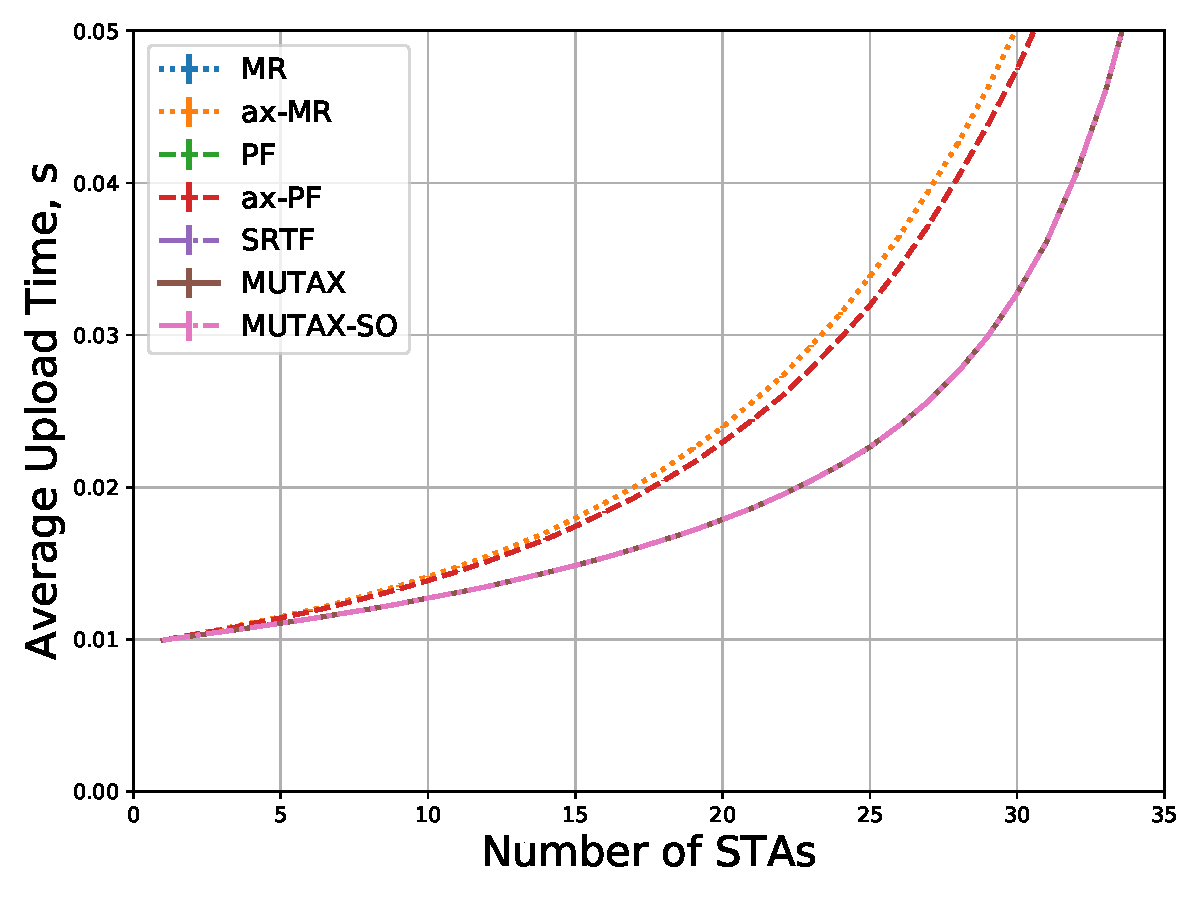
\includegraphics[width = 0.32\linewidth]{5-d.pdf}
	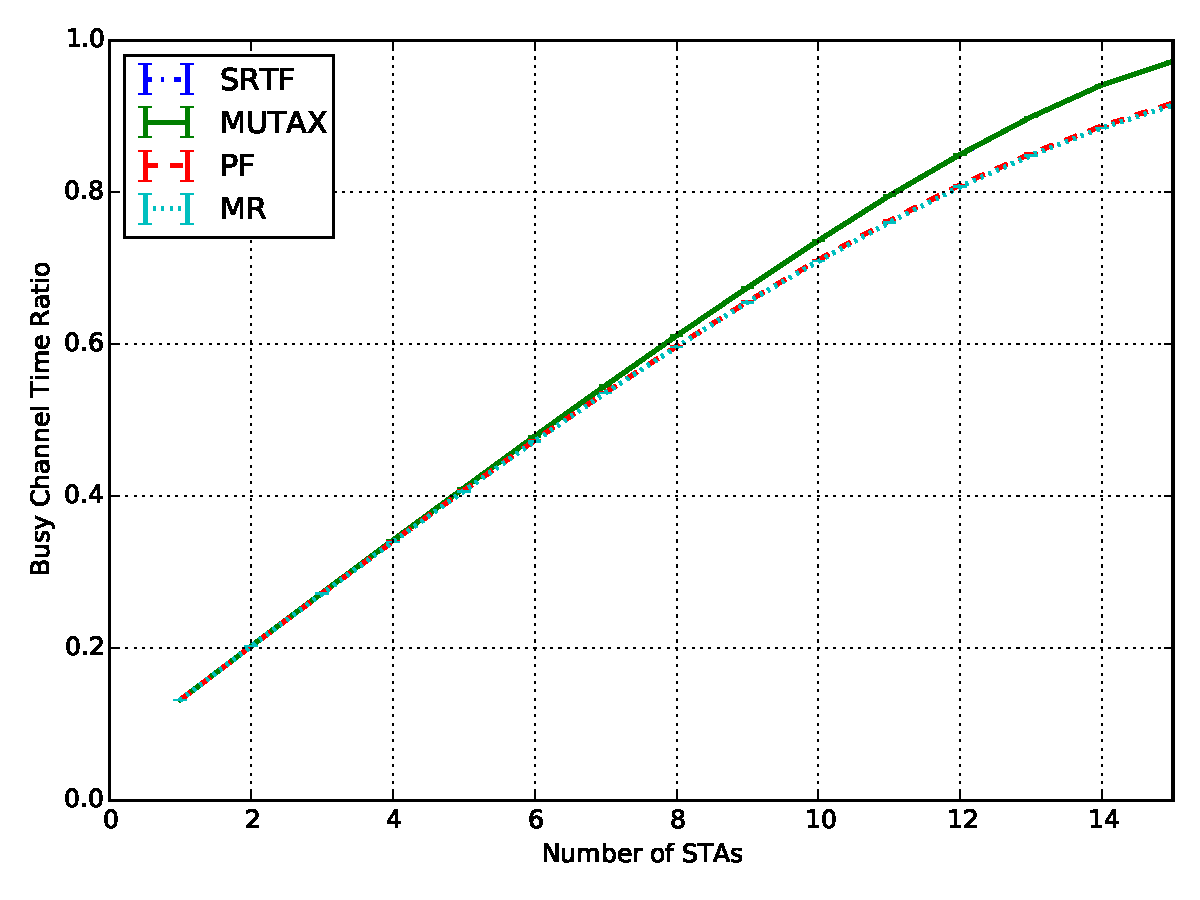
\includegraphics[width = 0.32\linewidth]{5-e.pdf}
	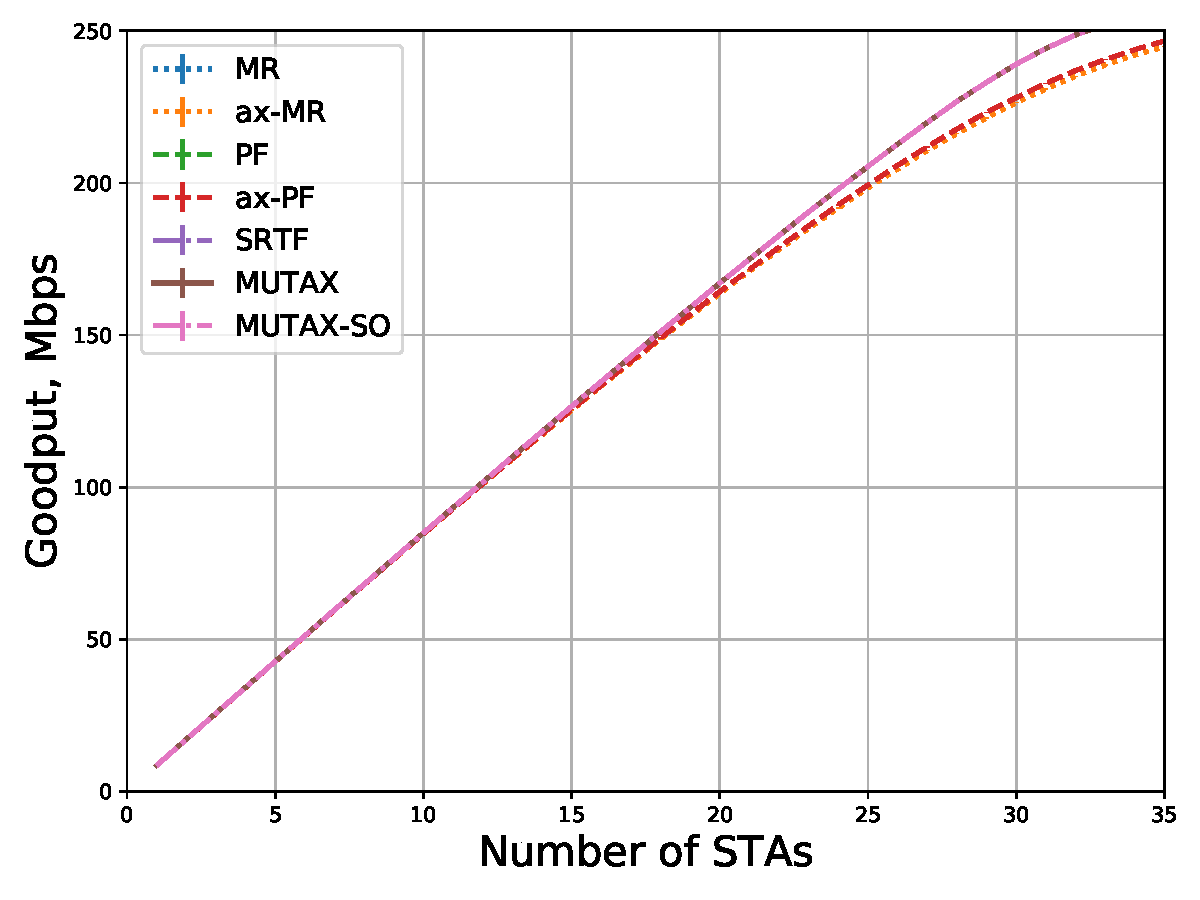
\includegraphics[width = 0.32\linewidth]{5-t.pdf}
	%\caption{\label{fig:10-d} Upload Time vs Number of STAs in the small circle.}
	%\end{figure*}
	%
	%\begin{figure}[tb]
	%\centering
	\caption{\label{fig:10-e}  Upload time, busy channel time ratio and goodput vs the number of STAs in the small circle.}
\end{figure*}

\begin{figure*}[bt]
	\centering
	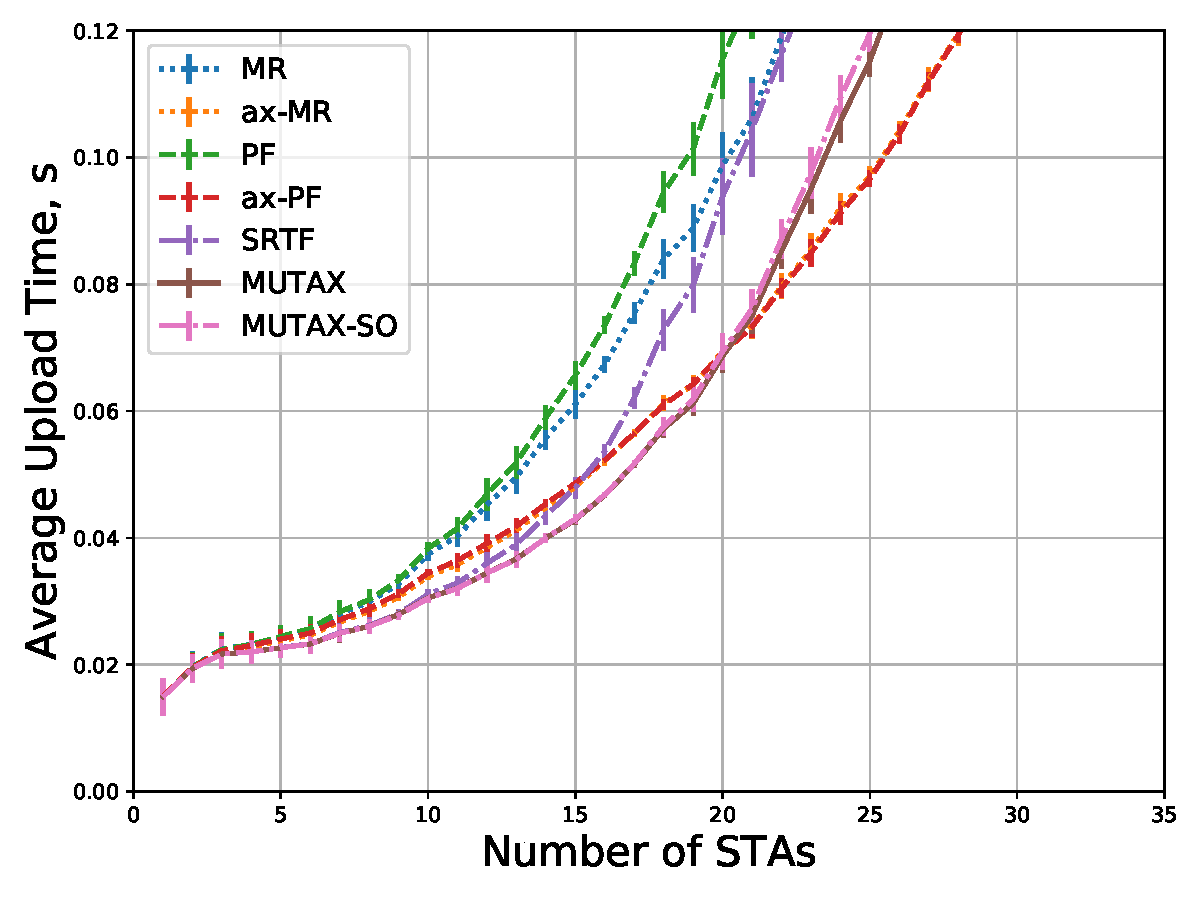
\includegraphics[width = 0.32\linewidth]{20-d.pdf}
	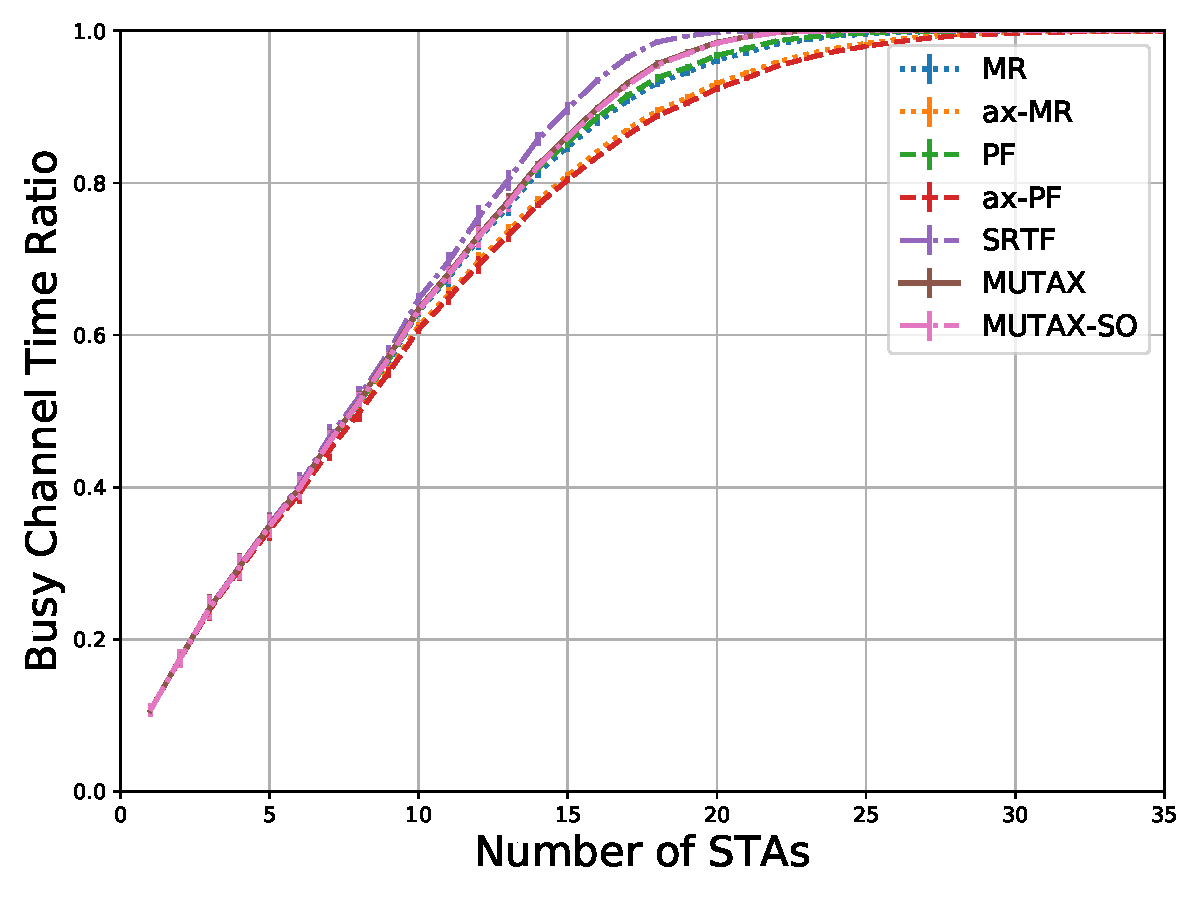
\includegraphics[width = 0.32\linewidth]{20-e.pdf}
	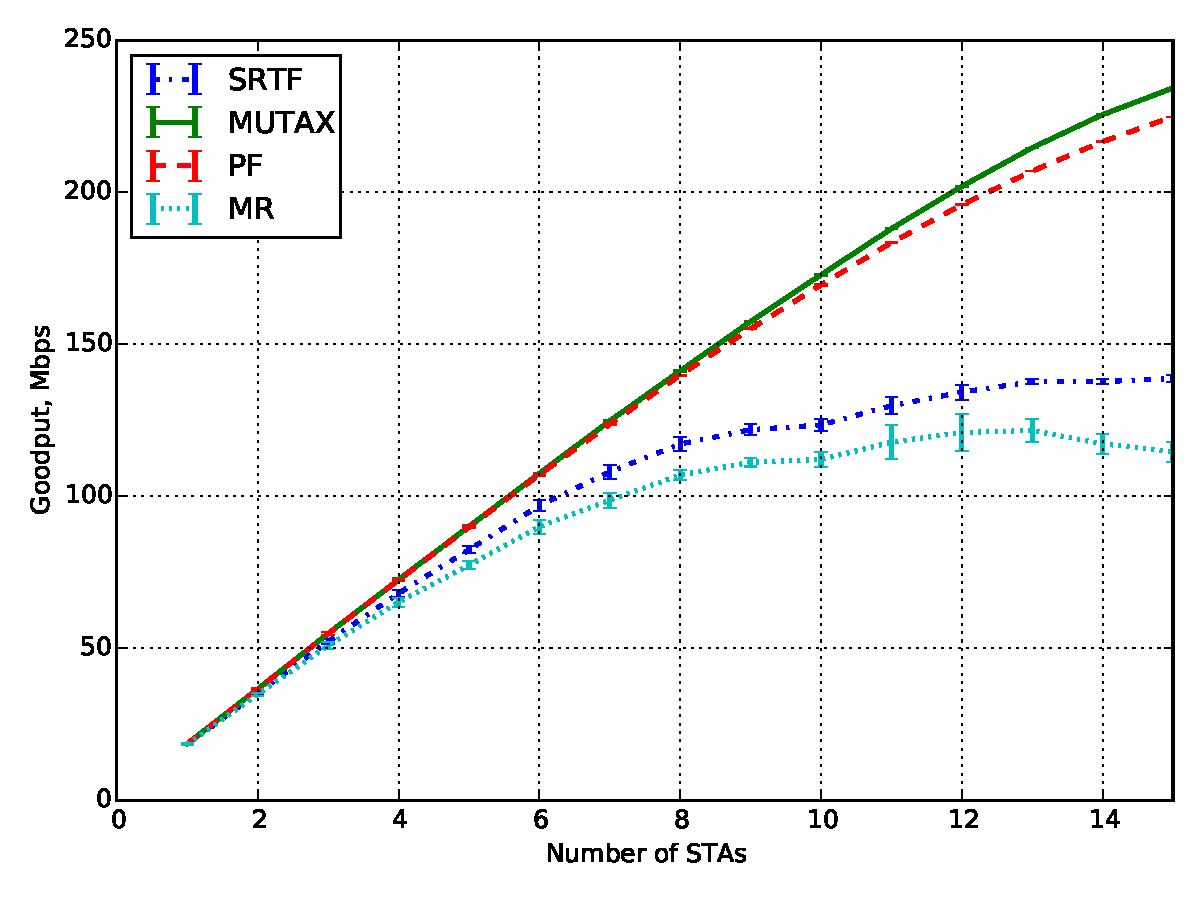
\includegraphics[width = 0.32\linewidth]{20-t.pdf}
	%\caption{\label{fig:25-d} Upload Time vs Number of STAs in the large circle.}
	%\end{figure}
	%
	%\begin{figure}[tb]
	%\centering
	\caption{\label{fig:25-e} Upload time, busy channel time ratio and goodput vs the number of STAs in the large circle.}
\end{figure*}

The second set of experiments corresponds to the case when STAs are located in a larger circle of radius $R = \SI{20}{\m}$.
Such conditions provide variety of MCSs among STAs and among RU widths, so it becomes feasible to split the channel between different users.
According to simulation results, see Fig. \ref{fig:25-e}, in this case designed to minimize upload time the classic SRTF work much worse than even 11ax adaptation of PF. At the same time, MUTAX shows 20\% lower upload time than PF. The results show that in this case the schedulers based on the exhaustive service (MR and SRTF) are  much less efficient than channel-splitting schedulers (MUTAX and PF) and the gap between them increases with the number of client STAs. %Note that MR and SRTF have a bit higher channel busy ratio than PF under higher load, since PF more intensively uses OFDMA and has lower overhead induces by headers and channel access.   
In a large circle scenario the gain in goodput of MUTAX against SRTF and MR is almost 100\%.


\section{Conclusion}
\label{conclusion}
In the paper, we have studied scheduling problem in IEEE 802.11ax networks, the standard of which is currently under development.
We show that because of 11ax OFDMA peculiarities the existing schedulers cannot be directly applied to the new technology.
Specifically, in the paper we have considered the problem of uplink scheduling which aims to minimize average upload time in a scenario with high number of active users.
We showed that depending on the scenario sometimes it is worth to use classic SRTF scheduler, while in other cases the channel should be split between several STAs in order to minimize upload time.
We develop a novel scheduler, called MUTAX, which adaptively chooses the best strategy and significantly outperforms existing popular solutions.

\bibliographystyle{IEEEtran}
\bibliography{biblio} 
\end{document}
